% Straight up stealing preamble from Eli Holmes 
%%%%%%%%%%%%%%%%%%%%%%%%%%%%%%%%%%%%%%START PREAMBLE THAT IS THE SAME FOR ALL EXAMPLES
\documentclass{article}

%Required: You must have these
\usepackage{Sweave}
\usepackage{graphicx}
\usepackage{tabularx}
\usepackage{hyperref}
\usepackage{natbib}
%\usepackage[backend=bibtex]{biblatex}
%Strongly recommended
  %put your figures in one place
 
%you'll want these for pretty captioning
\usepackage[small]{caption}

\setkeys{Gin}{width=0.8\textwidth}  %make the figs 50 perc textwidth
\setlength{\captionmargin}{30pt}
\setlength{\abovecaptionskip}{0pt}
\setlength{\belowcaptionskip}{10pt}
% manual for caption  http://www.dd.chalmers.se/latex/Docs/PDF/caption.pdf

%Optional: I like to muck with my margins and spacing in ways that LaTeX frowns on
%Here's how to do that
 \topmargin -1.5cm        
 \oddsidemargin -0.04cm   
 \evensidemargin -0.04cm  % same as oddsidemargin but for left-hand pages
 \textwidth 16.59cm
 \textheight 21.94cm 
 %\pagestyle{empty}       % Uncomment if don't want page numbers
 \parskip 7.2pt           % sets spacing between paragraphs
 %\renewcommand{\baselinestretch}{1.5} 	% Uncomment for 1.5 spacing between lines
\parindent 0pt% sets leading space for paragraphs
\usepackage{setspace}
%\doublespacing

%Optional: I like fancy headers
\usepackage{fancyhdr}
\pagestyle{fancy}
\fancyhead[LO]{How do climate change experiments actually change climate}
\fancyhead[RO]{2016}
 
%%%%%%%%%%%%%%%%%%%%%%%%%%%%%%%%%%%%%%END PREAMBLE THAT IS THE SAME FOR ALL EXAMPLES

%Start of the document
\begin{document}

% \SweaveOpts{concordance=TRUE}
 \bibliographystyle{/Users/aileneettinger/citations/Bibtex/styles/nature.bst}
\title{How do climate change experiments actually change climate?} % Paper 1/Large group paper from Reconciling Experimental and Observational Approaches for Climate Change Impacts

\author{A.K. Ettinger,I. Chuine, B. Cook, J. Dukes, A.M. Ellison, M.R. Johnston, A.M. Panetta,\\ C. Rollinson, Y. Vitasse, E. Wolkovich}
%\date{\today}
\maketitle  %put the fancy title on
%\tableofcontents      %add a table of contents
%\clearpage
%%%%%%%%%%%%%%%%%%%%%%%%%%%%%%%%%%%%%%%%%%%%%%%%%%%


\section* {Introduction}

\par Ongoing climatic changes are causing dramatic alterations to Earth's biota, increasingly altering the physiology, distribution, and abundance of organisms, and resulting in cascading community and ecosystem effects \citep{shukla1982,cox2000,thomas2004,parmesan2006,field2007,sheldon2011,urban2012}.  Much uncertainty remains, however, about how particular individuals, populations, species, communities, and ecosystems will respond as shifts in temperature and precipitation regimes become more extreme. Predicting these biological responses to current and future climate change, as well as how they will feedback to affect earth's climate and ecosystem services, are among the most significant challenges facing biologists today.
\par Researchers have sought to understand and forecast biological responses through a variety of strategies, including observational studies, model-based approaches, and experiments. Much work has focused on temperature because increased greenhouse gas emissions have a relatively straightforward effect on this climatic variable, at least as compared to precipitation \citep{ipcc2013}. Observational studies typically correlate observed biological patterns with trends in climate; however, it is challenging to disentangle the causal effect of warming from other factors that have also changed, such as successional stage or land use. In addition, future climate change is expected to result in conditions that are outside those that have been observed historically \citep{ohlemuller2006,williams2007,williams2007b,ipcc2013}. Modelling techniques can be useful in this regard, but these methods often rely on untested assumptions, for example, that climate limits performance \citep{pearson2004,ibanez2006,swab2012}. Experiments are therefore a critical component of the biologist's toolkit for understanding climate change impacts, and are often considered the ``gold standard" of knowledge \citep[e.g.][]{box1978,gelman2014}. In situ climate warming experiments allow effects of temperature and  precipitation to be isolated from other  environmental changes that can confound conclusions drawn from observational data sets. In addition, a range of warming  and precipitation treatments can be applied, such that potential non-linear responses may be evaluated. Compared with controlled growth-chamber experiments, field-based experiments offer the possibility of preserving important, but unknown or unquantified, in situ biotic and abiotic drivers and interactions. Climate change experiments in the field may therefore be able to elucidate many biological responses to future climate change.
\par Experimental climate manipulations take a variety of forms, manipulating temperature, precipitation, atmospheric CO2, and other variables using a wide range of techniques \citep{shaver2000,aronson2009}. In the field, temperature increases can be simulated using ``passive" warming infrastructure, such as open-top chambers, that trap energy already available in the environment, or ``active" warming methods, which heat ecosystems using external energy inputs  \citep[e.g. gas-powered forced air heaters, electrical-powered soil warming cables or infrared heaters][]{shaver2000}. Many field experiments have explored biological responses to interacting environmental changes: active warming methods have been combined with precipitation manipulations, (e.g. snow removal,  water additions and reductions), in  an  effort to create  climatic  conditions such  as  those  forecasted  under  future climate  change scenarios \citep [e.g.][]{price1998,cleland2006,sherry2007,rollinson2012}.
\par Seeking to prepare  for future, altered  biological conditions, scientists and others  often attempt to extrapolate the results of in situ climate change experiments to forecast how organisms and ecosystems will respond to particular climate change scenarios.  Even in cases where extrapolation is not the explicit goal of climate change experiments, these studies are often used to draw conclusions  about how anthropogenic warming  will affect species' performance  (e.g. growth and  survival)  and  distributions\citep{dukes1999,hobbie1999,reich2015,gruner2016}.  Despite these applications, a detailed  assessment of how different types of experimental warming alter the environmental conditions experienced by organisms, and the extent to which these conditions accurately simulate current field conditions and anticipated climate change, is lacking.  In addition comparing experimental results with observations and forecasts, there is a need to reconcile experimental results across the diverse methods, locations, and species to date. 

\par A detailed understanding of how climate change experiments actually alter climate is critical in order to realize the forecasting potential of climate change experiments. Here, we use  plot-level daily  microclimate  data  from  12 climate  change  experiments  that  manipulate temperature and precipitation to demonstrate the direct and indirect ways in which environmental conditions are altered  by active  warming technologies. We then highlight the challenges associated with quantifying and interpreting biological responses to these climate manipulations, and using these interpretations to forecast  more widespread responses to contemporary climate change. Finally,  we use findings from our synthesis to make recommendations for future  climate  change experiments.  We focus on in situ active warming  manipulations, because recent analyses indicate that active warming methods are the most controlled, consistent, and ``true to climate change predictions" \citep{kimball2005,kimball2008,aronson2009,wolkovich2012}. The data we use were collected between 1991 and 2014 from North American and European climate change experiments (Figure \ref{fig:map}) and  have been merged into a new, publicly  available  Climate from Climate Change Experiments (C3E) database (see Supplemental Materials  for details). 

%Not sure where to put this in: These advantages come at a cost, however.  Experimental in situ active climate  manipulations are logistically challenging  and expensive; it is difficult to design,  implement,  and  monitor  replicated experiments that consistently apply  the intended climate  manipulations \citep{aronson2009}.
%For supplement: we carried out a full literature review to identify all active field warming experiments then obtained daily (or sub-daily) climate data from as many as possible (we obtained data for 12/XX total identified experiments, see Supplemental Materials for details). We are thus able to show, for the first time, the complex ways that climate is altered by active warming treatments, both directly and indirectly. 
\section* {Complications in extrapolating experimental climate change}
Climate change experiments often include detailed monitoring of climate variables at the plot level, yielding large amounts of data, such as daily or hourly temperature and other climate variables, over the course of the experiment. However, biologists are generally interested primarily in the biological responses associated with each treatment (e.g. growth, abundance, or phenology of a species). Not surprisingly, then, authors typically provide detailed information on the observed biological responses, and report only the mean change in climate over the course of the experiment and whether or not that mean change matched their target level of change \citep[e.g.][]{price1998,clark2014a,clark2014b,rollinson2012}. 
%CRR: I think it's good that you mention we don't report the climate because we're interested in the organisms and it leads to a publication bias.  I don't know how to phrase it, but we (people that did the experiments) also often don't go into more detail because the experimental application can be very buggy with sensors going out, power outages, etc. and we've had to find that balance between accurately reporting our ecological story without going into the endless pits of study caveats.
\par Though the published focus is often on shifts in the mean, the imposed climate manipulations actually result in much more complex climatic shifts, for several reasons that we discuss in more detail below. First, in addition to shifting mean temperatures, experimental warming treatments may alter the temperature range and variance as well. Second, the magnitude of change in these manipulations is likely to vary in time and space. Third, the equipment required to conduct these manipulations can also alter climate at the plot level. All of these complications challenge our interpretation of how experimental warming studies can be applied to forecast effects of climate change, and we discuss them in more detail below.
\subsection* {Treatments alter the temperature range and variance, as well as the mean}
Warming treatments affect minimum and maximum temperatures in different ways, and also alter the variance in temperature. For example, we found that active warming increased minimum air temperature by, on average, 0.84 degrees C per degree of warming target, whereas maximum temperature increased only 0.51 degrees, on average, per degree of target warming. We also found higher coefficients of variation in air temperatures in actively warmed plots, compared with controls at the same sites in the same years. This was true for both minimum and maximum air temperatures (Figure \ref{fig:cv}). These differences in temperature range and variation, appear to be small, but they may be important. For example, even slight changes in temperature can alter critical biological thresholds, such as freeze-thaw cycles \citep{mcdaniel2014}. Other studies have also documented that warming treatments may affect diurnal versus night temperatures differently \citep{shen2016,matthews2016}. (Question for everyone (Lizzie/Ben/Miriam/Ann Marie/Aaron/Yann/Isabelle/Jeff/Christy): this paragraph needs help! I have had trouble coming up with a good figure to go with this point, and have found relatively small but significant differences in temperature range and coefficient of variation. Alternatively, do you think this paragraph should be cut?) 
%yann:I suggest that warming treatments also buffer extreme cold events. It would be nice to compare for instance minimum temperatures (or absolute minimum temperature) in spring between the control and the warming treatment and to see if this difference is bigger than between the mean or max temperature. I expect it to be much larger during cold night with clear sky due to radiative cooling in the control that is not occuring in the warming plot due to artificial warming...
\subsection* {Treatments vary over time}
The common practice of reporting only the mean temperature difference, across the duration of the study, may also hide variations in daily, seasonal, and annual temperatures among treatments. For example, as described above, warming treatments can cause decreases in the diurnal temperature range within experimental plots, compared with ambient conditions \citep{hoeppner2012}. This may be similar to what is projected for parts of world; however, this will likely vary spatially, as some regions have experienced higher daytime warming than nighttime warming, whereas others have experienced the opposite \citep{ipcc2013}. 

\par In addition to daily fluctuations, there are frequently strong seasonal variations in experimental warming effects (Figure \ref{fig:effwarm}). (Christy: Could you make some changes to this figure? See questions in caption of the figure). This may occur because treatments are not applied consistently over the year, either because heat applications are frequently shut off during some seasons such as when snow cover is present or because some heating methods, even if left on throughout the year, are not capable of applying consistent warming year-round \citep[e.g.][]{clark2014a,clark2014b,hagedorn2010}. For example, seasonal precipitation patterns can alter the effectiveness of warming treatments, since both infrared heaters and soil cables may fail to achieve the target temperatures during  rainstorms\citep{peterjohn1993,hoeppner2012}. Wind has also been shown to alter thermal efficiency of infrared heaters, so if heater capacity is limited, target warming levels may not be reached during windy conditions\citep{kimball2005,kimball2008}.
% CRR: Is this seasonal precip pattern related to the point about snow cover you mention earlier?  I'm wondering if there's some sort of snow or climatic threshold where warming has less of an impact.

\par Experimental warming effects can also vary across years  (Figure \ref{fig:blockyear}). This  can be due  to interactive effects of warming  treatments and  precipitation, wind, or other aspects of weather  that may  vary  annually, as well as seasonally, as discussed above. Of course, there is bound to be variation in the amount of warming at daily, seasonal, and annual scales as anthropogenic warming progresses, as well. We do not wish to suggest that experimental treatments must be consistent one hundred percent of the time, in order to be relevant. Rather, we wish to call attention to the fact that variations in warming treatments at daily, seasonal, and annual time scales are rarely analyzed explicitly.  It is unknown how divergent these annual, seasonal, and daily variations may be from real (i.e. non-experimental) climate patterns. To better understand this potential divergence, we need a detailed comparison of the variation present in climate change experiments to observations in non-experimental settings, as well as to projected future changes given expected greenhouse gas emissions.  

\subsection* {Treatments vary in space}
In addition to temporal variation, there can be spatial variation in experimental warming effects, such that extrapolation of experimental warming to forecast climate change impacts may not be a straightforward space-for-time substitution \citep{johnson2008,jochner2013}. For example, the C3E database contains three studies that used blocked designs, allowing us to examine spatial variation in the amount of warming (i.e. the difference between treatment and control plots within a block). We found that the amount of warming may vary by more than one degree among blocks (Figure \ref{fig:blockyear}, Table 1S), resulting in lower warming treatments that varied almost 100\% of their target temperature and higher warming treatments varying 20\% %(EMW: I am eye-balling, give exact values).% EMW: I offered one way to build on the finding, you could come up with many others instead -- I think it is important to just point it out a little more. 
\par There are numerous potential causes for these differences in warming levels among blocks, given the same warming treatment. It is possible that fine-scale variation in vegetation, slope, aspect, soil type, or other factors alter wind or soil moisture which in turn affect the thermal efficiency of heaters, or other aspects of the warming treatment, as discussed above\citep{peterjohn1993,kimball2005,kimball2008,hoeppner2012}.  In addition, fine-scale variation in the amount of sun received by a plot, perhaps due to vegetation cover or slope, may also affect temperature \citep{rollinson2015}. The observed differences in effective warming among blocks highlights the importance of quantifying temperature, soil moisture, and other climate variables at the plot scale, as well as a need to better understand how fine-scale variation in slope, vegetation, and other factors influence the microclimatic conditions experienced by organisms.  
\par Presumably, there will be spatial variation in future climate change effects, given that warming to date has varied spatially \citep{ipcc2013}).  Accurate extrapolation of climate change experiments may therefore depend on the extent to which experiments encompass a representative amount of existing natural variation (e.g. gradients in slope and aspect) present at the scale at which the extrapolation is being made. More detailed, fine-scaled comparisons of experimental and observational studies are necessary to better understand how this spatial variation in warming affects our interpretation of responses to warming. 
% CRR: There's some lit out there that talks about the geographical of bias of climate change research... I know some of it is related to flux tower location and I think some papers came out as NEON was getting rollign to justify their geographical approach

\subsection* {Experimental infrastructure alters climate}
The experimental structures themselves alter temperature and other important biotic and abiotic variables, in ways that are not generally examined or reported in experimental warming studies. The possible existence of these effects are widely acknowledged, and some studies include `shams' or `disturbance controls' in an attempt to account for them. However, the magnitude and implications of structural effects on climate are rarely discussed or interpreted in climate change studies.
\par To investigate the magnitude of these effects, we compared temperature and soil moisture data from five active warming studies at two sites: Duke Forest and Harvard Forest\citep{farnsworth1995,clark2014a, marchin2014, pelini2011}. These were the only studies in our database that included two types of control plots: structural controls (i.e. `shams' or `disturbance controls,' which contained all the warming infrastructure, such as soil cables or infrared heating units but with no heat applied) and ambient controls with no infrastructure added (see Supplemental Materials for details). Other studies include only the structural controls (n=3) or only the ambient controls (n=4).
%Is it worth pointing out the long history of such "cage controls" in marine intertidal and subtidal research that somehow has not translated to terrestrial research? Or would that be overkill?  

\par We found that experimental structures altered air and soil temperatures in opposing ways:  air temperatures were higher in the structural controls, compared with the ambient air with no structures installed, whereas soil temperatures were lower in the structural controls compared with ambient soil (Figure\ref{fig:shamamb}). This general pattern was consistent across the different temperature models we fit (mean, minimum, and maximum), although the magnitude varied across seasons (Figure \ref{fig:shamamb}), as well as among studies, years, and with ambient temperature (Table XS). Soil moisture was lower in structural controls compared with ambient conditions (Figure \ref{fig:shamamb_mois}). 
\par There are several possible mechanisms for the observed differences between ambient and structural controls. Elevated air temperatures in structural controls may be caused by infrastructure surfaces absorbing more solar radiation. For example, infrastructure materials may have higher heat capacity, higher emissivity, and/or lower albedo than the surrounding ground surface. In addition reduced air flow within the structures may lower evaporative cooling from structural control compared with ambient control plots. Although we could find very little discussion of measured temperature (or other) differences between ambient and structural control plots in most previously published work \citep[e.g.][]{farnsworth1995,pelini2011,clark2014a,clark2014b}, Clark et al (2014) do mention that ``control of the air temperature was less precise, in part due to air scooping on windy days." Marchin et al. (2015) also note that structural controls had mean spring air temperatures about 0.5°C or more above ambient temperatures. As for the differences in soil temperatures, it may be caused by alterations to heat capacity and emissivity in the structural materials compared to surrounding soil. Structures could also interfere with snow accumulation, thereby reducing snowpack and its insulation; this likely plays a bigger role at the Harvard Forest sites (exp04, exp07), where average snowfall is close to four feet, than at Duke Forest, where average snow accumulation is 7.5 inches or less. Peterjohn (1994) also reported cooler temperatures in structural versus ambient control plots, but only at shallow soil depths (4 cm deep, in their study). Similarly, in our analysis we found the greatest difference between soil temperature in sham and ambient controls to be in exp10, one of the two studies (the other was exp07) in which temperature was measured at depths of 2 cm, rather than 15 cm deep (exp03 and exp04). 
\par In addition to the structural effects that we document here on temperature and moisture, experimental structures may alter conditions by reducing light, intercepting precipitation, and altering herbivory and other biotic interactions\citep{kennedy1995,wolkovich2012}. Most warming experiments to date deal with this by calculating focal response variables relative to ambient control chambers to account for chamber effect\citep [e.g.][]{marchin2015}. Further documentation and analysis of the effects on abiotic and biotic factors, as well as in depth interpretation of how these effects may alter focal variables, is an important next step for climate change experimentation, particularly if we wish to apply results to forecasting. To date, these side effects are rarely reported or interpreted in climate change experiments, making them "demonic intrusions" in need of “eternal vigilance" to reduce\citep{hurlbert1984}. There will always be some artifacts present in any experiment, no matter how perfectly designed; we argue here for a better understanding of what those artifacts are in climate change experiments, and a fuller interpretation of how, if at all, they may affect translating the results of these experiments into forecasts. 
\section* {Secondary effects of climate change manipulations}
Climate change experiments often seek to manipulate one or two climate variables, such as temperature and precipitation. However, there are likely to be non-target abiotic and biotic factors that are also affected by these manipulations. For example, precipitation treatments typically reduce temperatures in climate change manipulations\citep{sherry2007,rollinson2012,mcdaniel2014}. McDaniel et al. (2014) observed that a twenty percent increase in precipitation reduced mean hourly temperatures by 0.3 degrees Celsius over the course of their two-year experiment. The magnitude of this effect can vary in space and time, however (Figure \ref{fig:effwarm}). 
\par In addition, experimental warming typically reduces vapor pressure deficit and soil water content (Figure \ref{fig:mois}),\citep[e.g.][]{sherry2007,morin2010,templer2016}. Of the twelve experiments in the C3E database, ten measured and reported soil moisture, and five measured air and soil temperature in addition to soil moisture. We found that soil moisture was reduced by 0.2 percent, on average, per degree of air warming (Table XS). While active warming experiments rarely manipulate soil moisture directly, soil moisture is unavoidably affected by changing temperatures. Because soil moisture is one of the most fundamental quantities affecting plant physiological functioning (Lambers et al. 2008) and climate system cycles of water and energy (Seneviratne et al. 2010), consideration of its alteration by experimental warming is vital. 
\par (Miriam: I redid your models, to match the structure of the other models in the paper: with site and year (nested within site) as random effects. This changed the results slightly. Could you work on this paragraph a bit, and add some interpretation with the new model structure and results?) %Miriam's text:We applied linear mixed effects models to analyze the effects of temperature treatment on soil moisture in those five experiments. We used year and site as random effects to account for variation in yearly climate and warming protocols, infrastructure, and depth of soil moisture measurement among sites. Candidate fixed effects were air and soil temperature minima, maxima, and means, though we constrained models to use only one soil and one air temperature variable to minimize predictor collinearity. Season and day of year were included in all models to account for temporal variation in the data, and models were distinguished by AIC scores. The most parsimonious model had mean air temperature and maximum soil temperature as explanatory variables; both significantly affected soil moisture. Soil temperature, predictably, was inversely related to soil moisture: a one degree (ºC) increase in maximum soil temperature yielded a modeled decline in soil volumetric water content of 0.0028 (1.7 percent of the median soil moisture across all sites and treatments). Surprisingly, however, air temperature was slightly positively related to soil moisture: a one degree increase in mean air temperature was associated with an increase in soil volumetric water content of 0.00071. Potentially, this result could be explained by the closing of plant stomata in response higher air temperatures (and therefore a higher vapor pressure deficit); this would decrease the gradient between soil and leaf water concentration, resulting in comparatively less water being pulled from the soil \citep{williams2015}.
\par Warming and precipitation treatments, and their indirect effects on abiotic factors such as soil moisture, can also alter the biotic environment, which in turn can produce additional secondary effects that alter climate. For example, Rollinson et al (2010) reported that tree composition shifted after three years of warming and modified precipitation treatments \citep{rollinson2012}. These shifts in composition may change competitive dynamics and, in turn, affect resource levels, such as moisture in the soil. In addition, given that warming reduces soil water content, it is likely to affect soil microbial communities, and therefore available nutrients as well. The magnitude of all of these effects are also likely to vary in space and time; some may be transient whereas others may be more permanent. 
%Could also add something about shrubs, which can also shade soil, and might be worth saying something more specific about how transient (or not) some of the resource limitation may be (e.g. nitrogen cycling) because some experiments (Harvard Forest, boreal warming in AK?) show very different patterns between first couple years and longer-term dynamics?
\par It can be difficult to tease apart the specific abiotic and biotic drivers climatic conditions in climate change experiments, but understanding the effects of an experimental treatment on these interrelated variables is critical when trying to determine mechanistic explanations for observed responses to warming. Even when experimental artifacts are introduced (such as artificial drying of soils or altered plant composition, due to experimental structures), if these secondary effects are quantified, they can be helpful in understanding how abiotic and biotic factors interact to affect physiological responses. For example, we can learn about the controls on stomatal conductance when the normal covariance between temperature, humidity, and soil moisture is altered. 
\par The widespread presence of unintended secondary effects of climate change manipulations highlight the importance of measuring environmental conditions at the plot level, and of using these measurements in data analysis and interpretation of results. Many climate change experiments (seven of the 12 in the C3E database, for example) model warming and/or precipitation treatments as categorical predictors (and in some cases, orthogonal crossed treatments, when both treatments are included in the experiment, i.e. a traditional repeated measures, three-way ANOVA). The interacting and secondary effects of these manipulations, as well as the plot-level variation in warming effectiveness and effects of experimental structures on temperature and soil moisture that we discuss above, demonstrate a clear need for an alternative modelling approach to fully understand the experimental results. One option is to include the continuous climate data (e.g. mean temperature over the study period) for each plot, as a predictor of the focal response variable, such as phenological state or species density \citep [e.g.][]{marchin2015, pelini2014}. A challenge with this approach is that much of the true variation in the climate is lost through aggregation (e.g. calculating mean annual or seasonal temperature), and chosen method of aggregation affects both the mean and variance of the climate estimate \citep [e.g.][]{clark2014b}. It may not be obvious which method of aggregation, or which combination of aggregated climate variables, is most appropriate, and this will likely depend on the response variable of interest. In these cases, model selection approaches have been used to identify the climate aggregation method that best explains the focal response\citep [e.g.][]{morin2010}. Alternatively, a continuous development model can be used to capture the full range of variation present in a climatic variable during the study period \citep [e.g.][]{clark2014b}.
\section* {Biological implications}
%In this section, it is important that we make strong links between the unreported statistics that we just described (seasonal and temporal variation, secondary effects) and potential biological responses.  I feed that as it is written right now, it is more a summary of just the biological responses with not enough emphasis on now they relate to better microclimate reporting.
% At ESA a couple years ago I saw a guy gave a talk showing how the different day/night warming impacted arthopod communities (they enclosured warming experiments with different diurnal warming patterns).  I wish i remembered the name, but will try to remember to search around for it... I think it was a student/postdoc with Oswald Schmitz (Yale). AE:sounds cool and relevant! couldn't find it.
\par We have highlighted a suite of factors that complicate interpretations of warming experiments. We argue that these largely unintended alterations are important for scientists to fully understand and report in their research (Figure \ref{fig:biolimp}). This is especially important because unintended climate alterations are likely to have biological implications, including for many of the major responses studied in warming experiments. Below, we discuss three example biological responses often studied in climate change experiments (plant phenology, plant growth, and soil respiration), for which indirect effects of treatments may have important implications. We argue that the interpretation of how these responses are affected by climate change is likely to be altered by using fine-scale, measured climate as the explanatory variables (e.g.. plot-level temperature and soil moisture), rather than by using the intended climate treatments (i.e. categorical comparisons or target warming levels). This is because detailed examination of multiple microclimate variables will allow a more complete understanding of the indirect, as well as direct, effects of applied treatments on a suite of abiotic and biotic drivers of focal responses.
\par Shifted plant phenology has been a focal response in climate change experiments experiments. Yet understanding exactly what drives shifted phenology may be more complicated than simply comparing shifts to the direct warming effects of the experiment. This is because phenology is likely to be altered in opposing ways by the increased air temperatures---which generally advance phenology \citep{wolkovich2012}---and decreased soil moisture---which may delay phenology or at least reduce advancement due to warming \citep{penuelas2004,craine2012,matthews2016}---characterized by warming treatments. Indeed, these opposing drivers may be responsible for the observed discrepancy between observational and experimental phenology responses to warming \citep{wolkovich2012}. However, observed effects of precipitation treatments on phenology have been variable to date, and remain poorly understood, perhaps because many previous studies have used the applied treatments, rather than the measured microclimate variables, as predictors in analyses \citep[but see][]{morin2010}. Climate change experiments that manipulate and measure air or soil temperature and soil moisture levels can be used to estimate effect sizes for these two climate variables and potential interactive effects of them on phenology. In addition, plant phenology responds to minimum temperatures, as well as mean and maxima \citep{shen2016,fu2016,piao2015}. This may also play a role in the discrepancy between observational and experimental studies, since diurnal versus night temperatures are affected differently by warming treatments\citep{shen2016,matthews2016}. 
\par Plant growth is also likely to be altered in opposing ways by the increased air temperatures and decreased soil moisture levels in experimentally warmed plots. For example, with warming and decreased vapor pressure deficit, stomata closure may reduce sapflow and growth \citep{templer2016}. Even small shifts in temperature may have a big effect, since the photosynthetic response to temperature is nonlinear \citep{berry1980}. Climate change experiments offer the opportunity to get these (and other) physiological measurements from a wide range of temperature conditions, which is essential for improving accuracy of ecosystem models and their forecasts.  %Do we need this last sentence? And/or need more here? Christy says: Many of these models use Berry's equations, but we're often relying on space-for-time studies to get us the responses of the tails of the distributions rather than seeing how organisms respond to the tails in the same locaitons. 

\par Direct and indirect effects of climate change experiments are also likely to affect soil respiration in ways that may alter carbon dynamics and net mineralization and therefore have other cascading effects that may or may not be realistic \citep{deltoro2015}. . For example, a meta-analysis based on studies using different warming techniques found that soil warming significantly increased soil respiration rate, net nitrogen mineralization rate and plant productivity, especially in temperate forest ecosystems \citep {rustad2001}. The amount of increase in these important ecosystem properties is likely to vary dramatically, depending on experimental methods. Warming treatments that are not applied year around \citep[e.g.][]{clark2014a,clark2014b} may result in effects that differ from those under consistent warming, since microbial communities that have strong effects on nutrient availability and soil moisture may be differentially affected by warming during summer versus during winter, when temperatures are close to critical cold thresholds and when the frequency of freeze-thaw events are likely to be altered\citep{rivkina2000,mcdaniel2014}. Furthermore, nutrient availability will then alter plant growth, a common focal response in climate change experiments: even a relatively small amount of newly available nitrogen from the soil could result in a substantial increase in carbon storage in woody tissues, especially if it becomes available during critical growth periods for plants. \citep{fatichi2014} YANN- Is this the correct citation? In addition, warming of soil versus air is likely to result in different effects on plant-soil microbe interactions, since soil warming experiments may increase net mineralization in early spring or winter, but plant phenology would be unlikely to advance in concert, unless additional air warming were applied \citep{du2014}.
These kinds of trophic mismatches may be present in climate change experiments, even if they are not expected to occur under natural warming \citep{kharouba2015}. 
\par Other biotic interactions are also likely to be affected by direct and indirect affects of climate change treatments. For example, Hoeppner and Dukes (2012) found that rodent disturbance varied by warming treatment (as well as year) in their climate change experiment. Insect diversity and community structure can change with active warming, and may have secondary effects on plants or other interacting organisms\citep{pelini2014,diamond2016}. A critical question is the extent to which these shifts in biotic interactions (and their effects on focal responses) are accurate forecasts of future shifts that are likely to occur with climate change, or due to side-effects that are unlikely to occur outside of experimental systems \citep{diamond2013}.

\section*{Recommendations for future climate change experiments}
 \par Climate change experiments provide invaluable information about biological responses to climate change, yet our results highlight that we do not fully explore the ways in which these climate change experiments are actually altering climate. These complications should not suggest that experimental climate change studies offer little value. Instead, we believe these complications and the related climate data provide the foundation to designing better experiments and gaining the most knowledge and utility from existing experiments. Below we describe recommendations to improve implementation, interpretation, and communication of climate change experiments in the future.
\par\textit{Include both structural and ambient controls} and collect, use, and report data collected within them. Fewer than half of the studies in our C3E database included these two control types and monitored climate within them (5 out of 12); all experiments showed significant effects of shams. As far as we know, only one of the studies in the database monitored both climate and focal biological response variables in both types of controls, however \citep[ e.g. plant phenology][]{marchin2014}. Future monitoring of all climate and biological variables in both control types will enable scientists to tease apart mechanisms due to experimental design from mechanisms due to actual shifts in climate.  
\par\textit{Maximize the length of climate change experiments} by running them for as long as possible. This will allow study of how inter-annual variations interact with climate change treatments, especially when looking at non-linear and mulch-year processes such as phenology. It will also allow us to understand how long-term responses may differ from  transient ones \citep{franklin1989,giasson2013}. 
\par\textit{Collect fine-scale climate data}, at least twice daily, and ideally hourly, to allow for minimum and maximum values, as well as critical thresholds, such as the number and duration of freeze-thaw events and accumulated chilling hours, to be to be analyzed and interpreted, in addition to mean values \citep{mcdaniel2014}. In assessing the frequency of measurements, it is critical to consider the chronobiology of the event and organisms of interest. For ants, this might mean that temperatures be monitored at the frequency of minute (Aaron: do you have a citation for this); for bacteria, even more frequently.
\par\textit{Analyze continuous, plot-level climate variables}, rather than discrete treatments (i.e. ANOVAs). There can be substantial variation among plots in effects of warming and precipitation treatments (Figure \ref{fig:effwarm})). Furthermore, these two treatments are not independent: precipitation treatments alter the effectiveness and warming, and warming treatments alter available moisture levels. Analyzing climate in this way will allow much more in-depth understanding of the drivers and effects of variation in temperature and moisture.
\par\textit{Consult observational records and forecasts to design relevant manipulations}. If the goal is to mimic future climate conditions, careful consultation of climate change projections for the study region, as well as historical data, can aid in selection of warming and precipitation treatment methods that most closely mimic anticipated changes. When it is not possible to match anticipated changes in climate, studies should report how imposed treatments compared to projected changes. In addition, the timing of the imposed treatments should be carefully considered, and ideally should match forecasts. If it is not possible to apply continuous treatments throughout the study, the seasonality and timing of treatments should be explicitly reported and the climate should be monitored throughout, even if no manipulations are implemented. In addition to designing experiments that shift mean climatic conditions, scientists should be thoughtful about what other aspects of microclimate are being altered, such as the minimum, maximum, variance, distribution, and critical threshold values. In particular, extremes can often have out-sized effects compared to shifts only in the mean state (Ben could you add a citation here).
%Do we want to add a recommendation to the list below that suggests selecting a scale of climate manipulation appropriate to the desired predictive power?  I’m thinking that we want to have a suggestion about capturing enough natural variation (in biotic community, topography, aspect, etc) for results to be predicative over a larger spatial scale.  
\par\textit{Publish high quality, usable data and metadata} such that data can easily be shared and used by others. In the metadata, report the number and cause of missing data points for climate, especially those collected in warming treatments. (For example, are data missing because the heaters failed, or because sensors failed) Report the timing of applied warming treatments (i.e. exact start and end dates, within and across years), as well as variations in daytime and nighttime and seasonal variations in climate variables. Given that experimental in situ active climate  manipulations are logistically challenging  and expensive \citep{aronson2009}, and that they often produce a large volume of fine-scale climate data, good curation and data sharing will ensure wider use and more in-depth understanding of these valuable data. 
\par\textit{Consider implementing and following community standards for reporting climate data} 
When studying biological implications of a global challenge as large as climate change, it will facilitate progress if we can design, run, and report experiments in such a way that we can eventually create a global data set. This recommendation stems from our work gathering and analyzing data from many climate change experiments. We found that studies report a diverse range of climate variables, collected in different ways (e.g. in the the C3E database, soil temperature was collected at depths ranging from 2 to 25 cm and soil moisture was collected at depths ranging from 8 to 30 cm, using different units and methods). It has been difficult to synthesize these data in a comprehensive way that can fully address important questions, and it will be a challenge to tease apart whether variable findings are due to methodological differences, to measurement error, or to true variation in biological responses. Question for everyone (Lizzie/Ben/Miriam/Ann Marie/Aaron/Yann/Isabelle/Jeff/Christy): I'm not sure if i want to keep this recommendation- perhaps its the part of me with libertarian/anti-top-down tendencies (although i can certainly see the value in this). What do others think?

\par Documenting biological impacts of climate change has over a 20 year history in ecology today. During this time, in situ field experiments have been critical in making the mechanistic link between warming and a number of major biological impacts, such as changes in productivity, soil respiration, the phenology of plant and animals, and shifted community and ecosystem dynamics. Yet, as climate change across the globe continues with projected warming likely to exceed 2 degrees Celsius over the next 80 years \citep{ipcc2013}, ecologists are challenged to not only document impacts but make quantitative robust predictions. Our ability to meet this challenge requires building on the data from current and past experiments to best understand how changes in climate alter ecological processes, and to build better experiments in the future. As a first step, we have compiled the first database of fine-scale climate data from multiple warming experiments and shown how time, space and artifacts may hinder simple interpretations of climate change experiments. The next steps require the ecological community to build on these data and their findings to develop and use new approaches in future experiments. This will provide more accurate estimates of altered climate in these experiments and in turn, more accurate estimates of critical biological changes. 
\bibliography{/Users/aileneettinger/citations/Bibtex/mylibrary}
\clearpage
\section* {Figures}
\begin{figure}[p]
\centering
 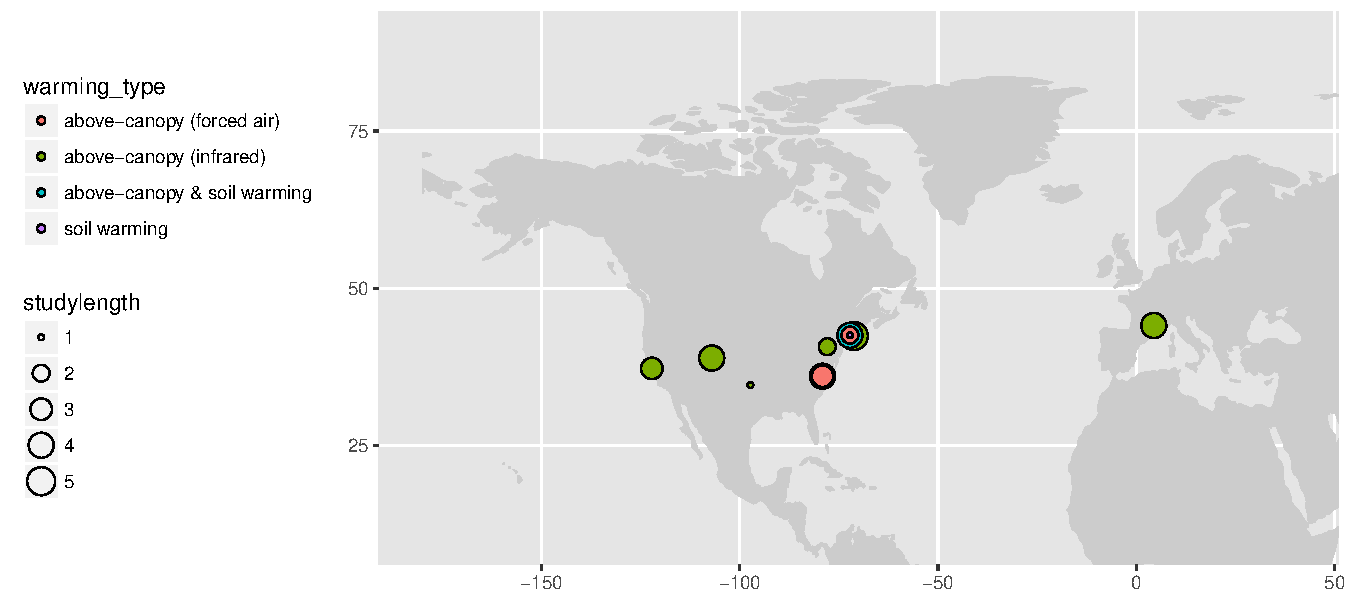
\includegraphics{../Analyses/maps/expsites.pdf}  
\caption{DRAFT Map of experimental sites in C3E datbase. Question for everyone (Lizzie/Ben/Miriam/Ann Marie/Aaron/Yann/Isabelle/Jeff/Christy): Does anyone want to volunteer to make a beautiful new version?} 
\label{fig:map}
\end{figure}
 \begin{figure}[p]
 \centering
 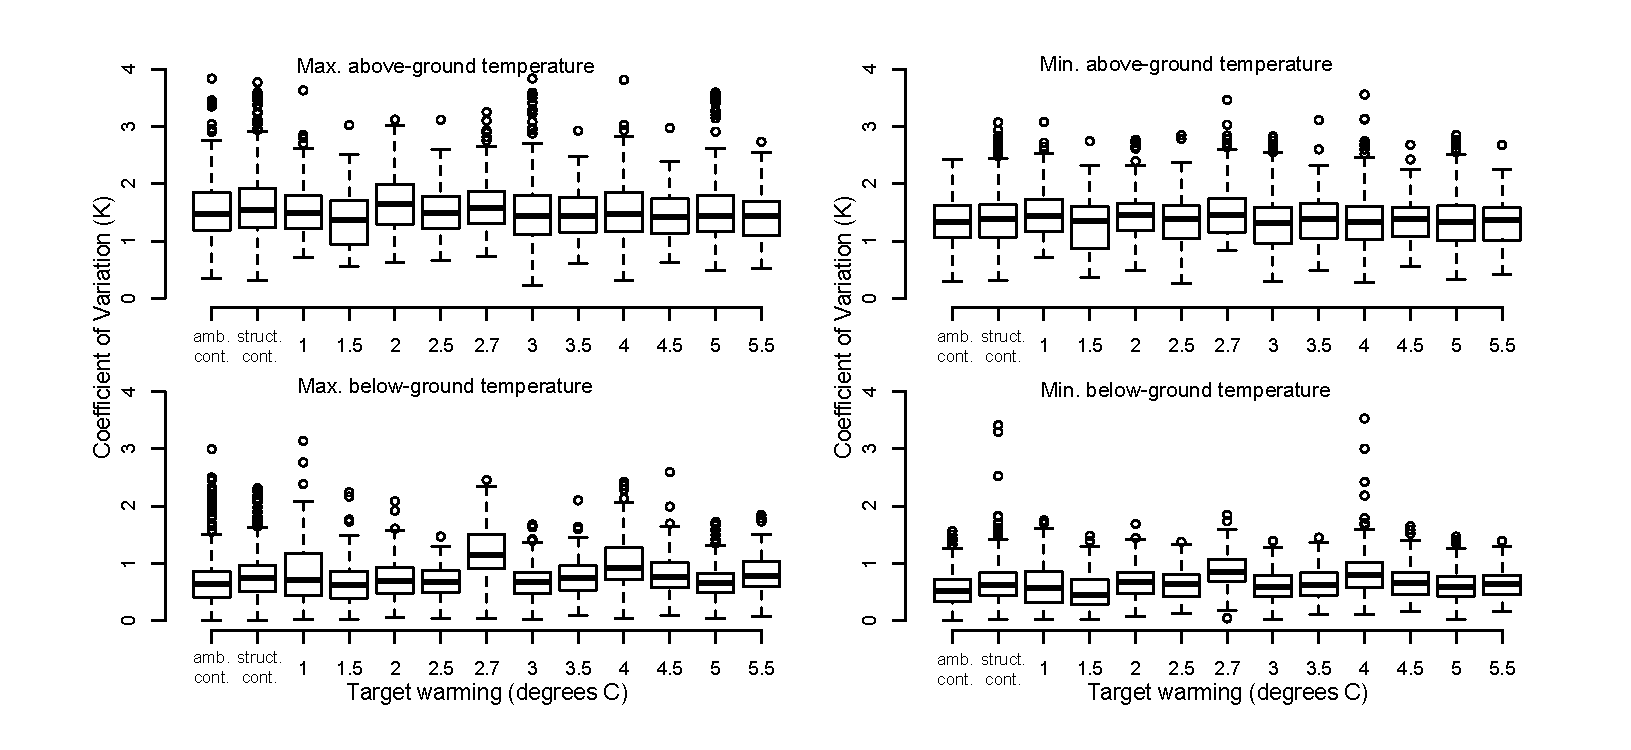
\includegraphics{../Analyses/figures/DRAFT_CVBytreatment.pdf} 
 \caption{Ambient controls have reduced variation, compared with structural controls and nearly all warming treatments. I'm not happy with this figure- I've tried so many different ways of showing the (small but) significant differences in temperature range/variance among ambient controls, structural constrols and warming treatments, in addition to the statistical analyses described in the text and supplement. Question for everyone (Lizzie/Ben/Miriam/Ann Marie/Aaron/Yann/Isabelle/Jeff/Christy): I need help with ideas for other ways to show this, or thoughts on if the point should be dropped, since the differences are minor and hard to see.} 
 \label{fig:cv}
 \end{figure}
\clearpage
\begin{figure}[h]
     \centering
 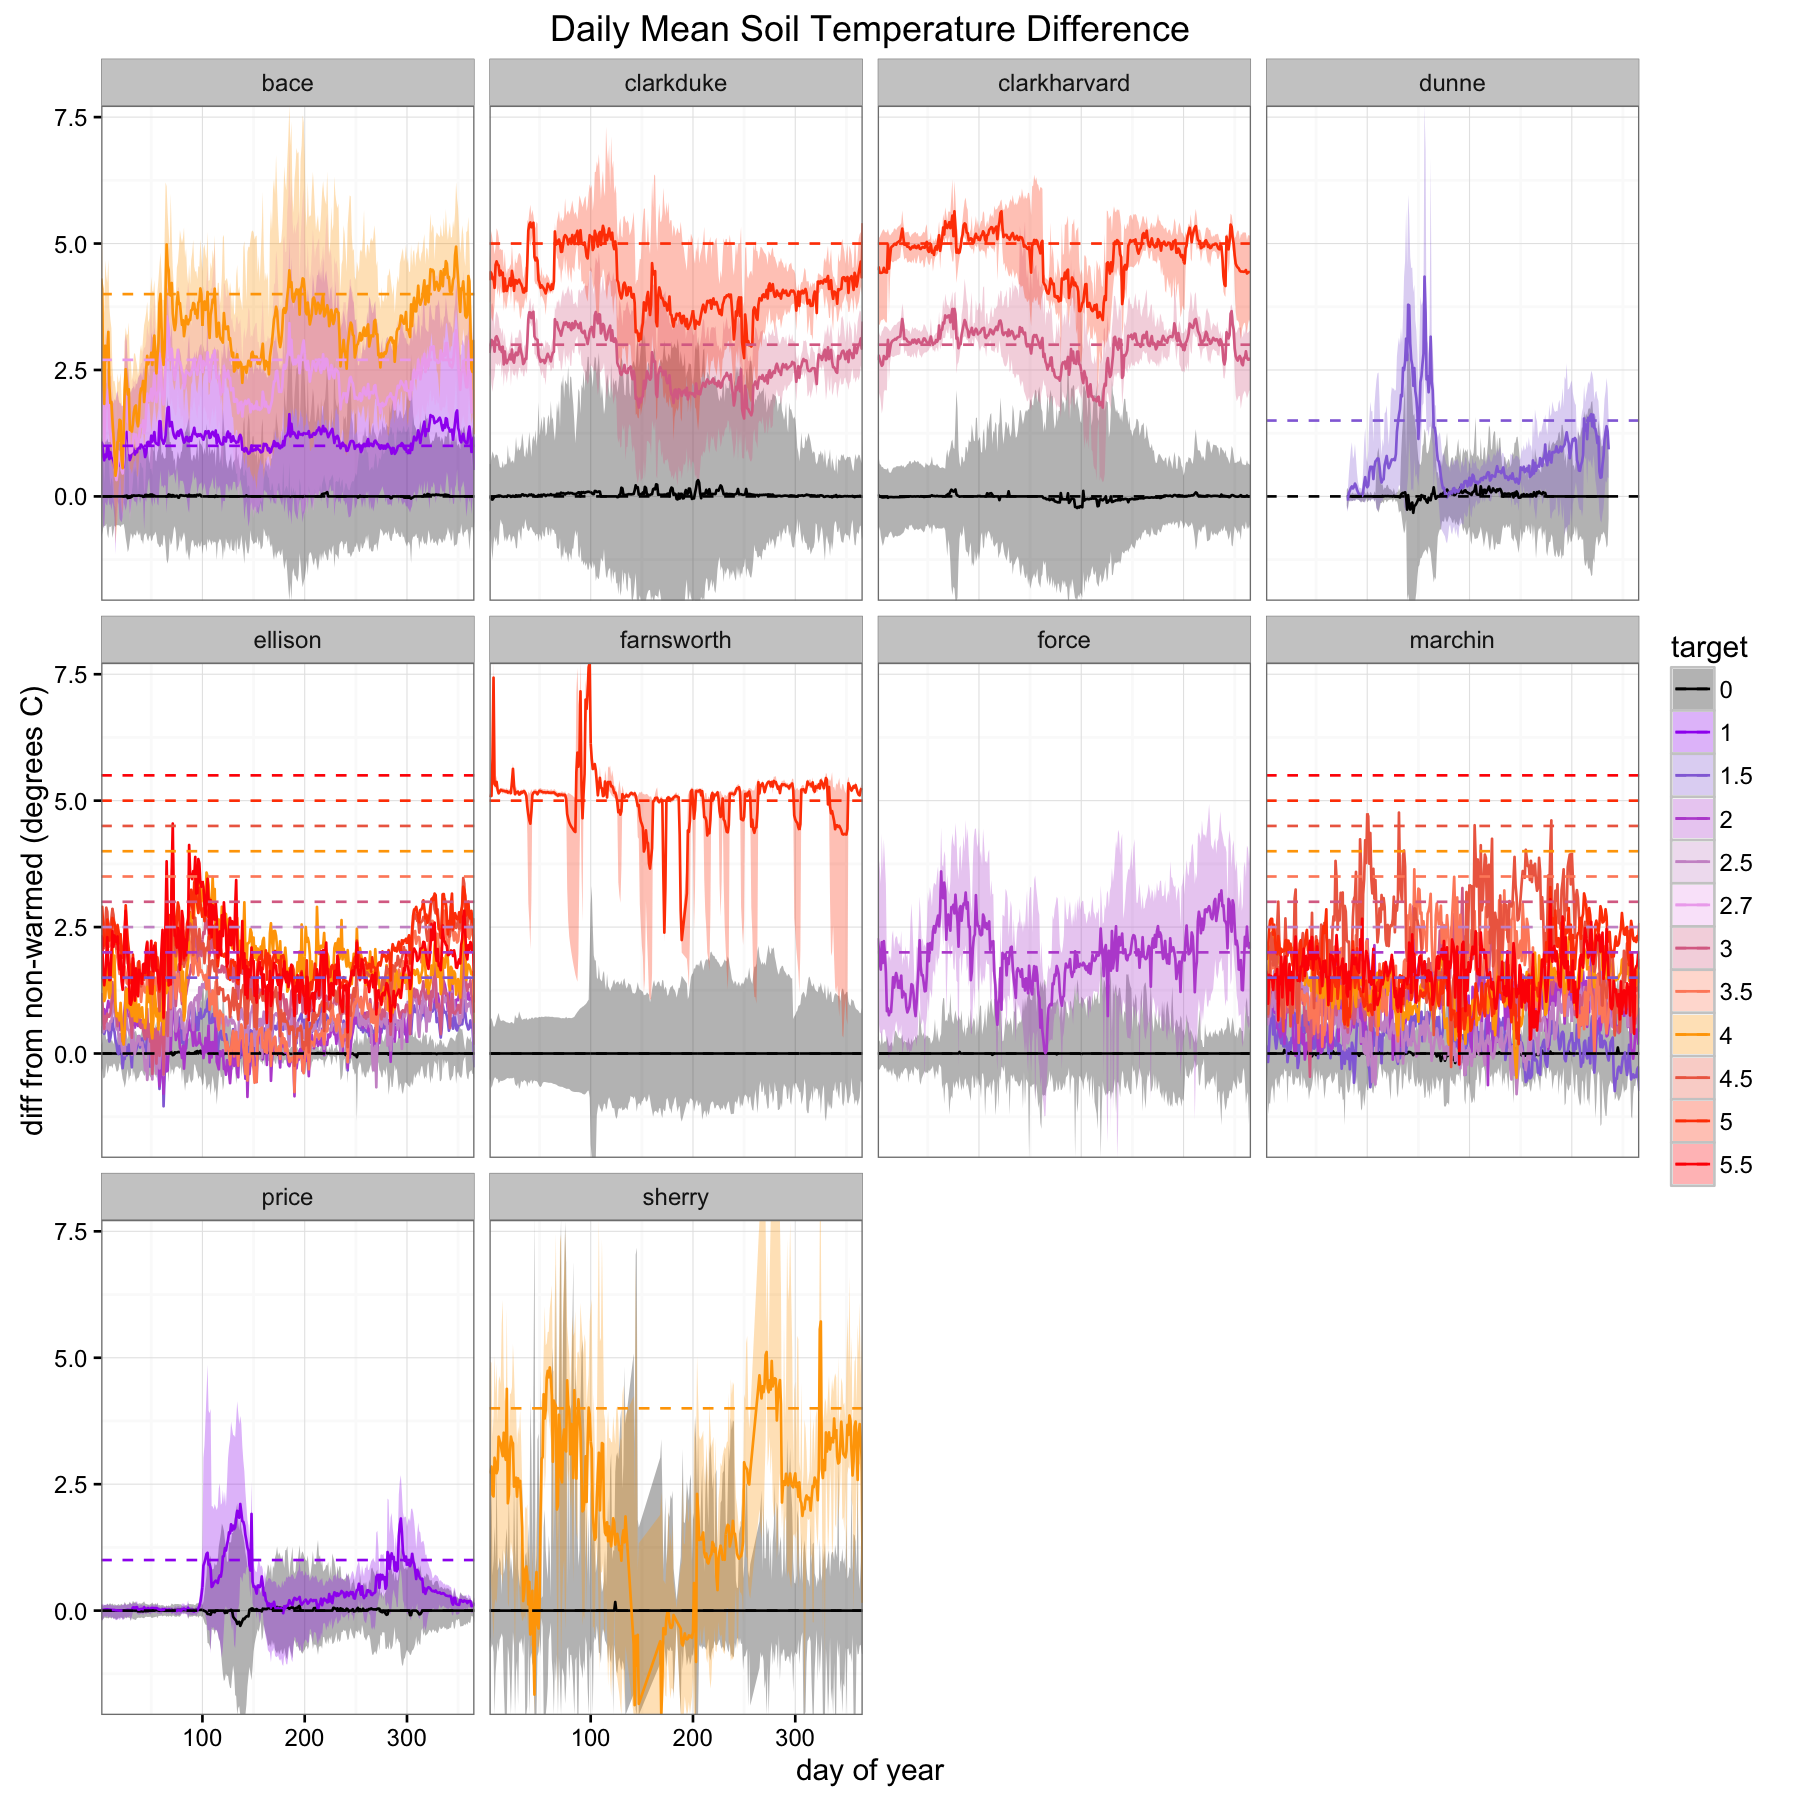
\includegraphics{../Analyses/figures/Exploratory_TimeSeries_SoilTemp1Mean_Deviation.png}
 \caption{Time series of deviations from mean soil temperature over one year, in control (black line) and warming treatments with various target warming levels at 10 study sites. Christy: could you add the mean annual temperature somehow to each panel- just so that we can see the variation among sites? Also, I am wondering if you could modify the code to make these estimates for each year of a study, as well as overall. I also was not quite sure if this represents a summary of deviations across all years, if studies were multiple years, or just one year? Please write a brief summary of these analyses- probably for the supplemental.}
  \label{fig:effwarm}

 \end{figure}
\begin{figure}[h]
     \centering
 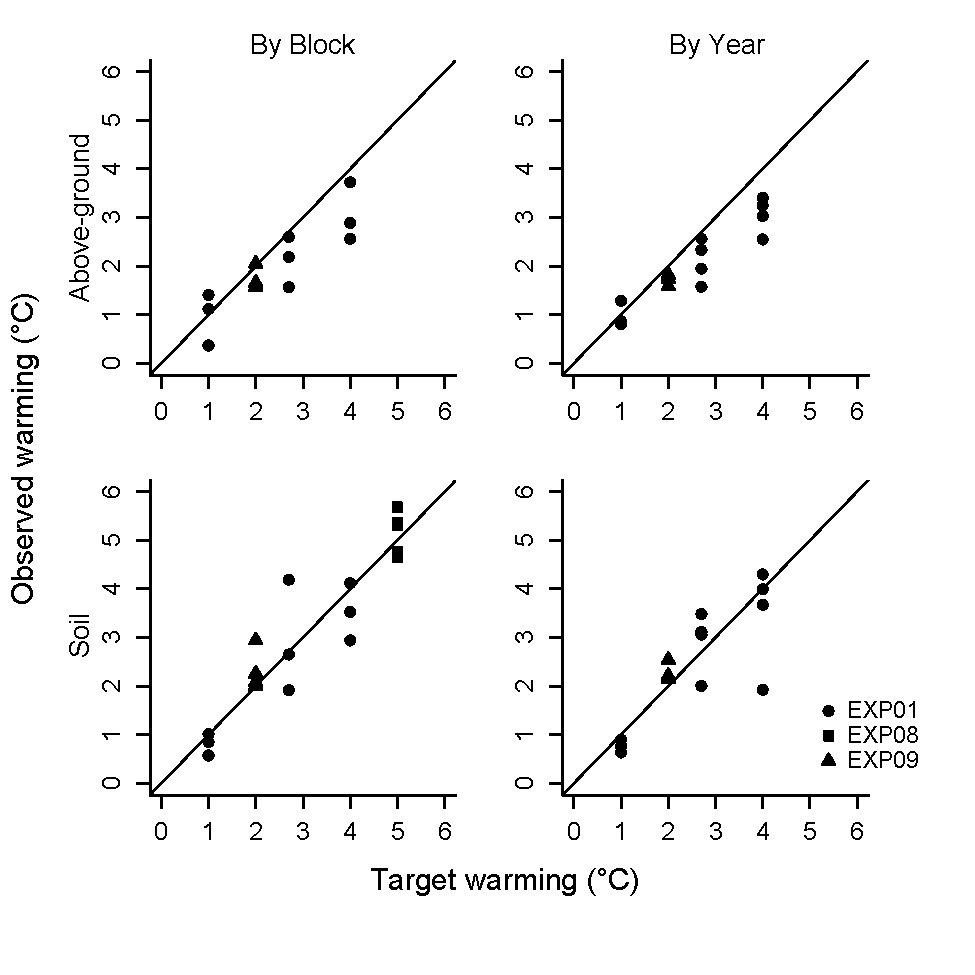
\includegraphics{../Analyses/figures/BothWarmingbyblockyear.pdf}    
 \caption{The amount of observed warming (i.e. the difference between treatment and control plots, within each block) varies among blocks (left panels), as well as among years (right panels). Black line represents a 1 to 1 ratio (i.e. when observed warming is exactly equal to target warming). See Tables XS and XS for statistical differences.}
  \label{fig:blockyear}

 \end{figure}
\clearpage
 \begin{figure}[h]
\centering
 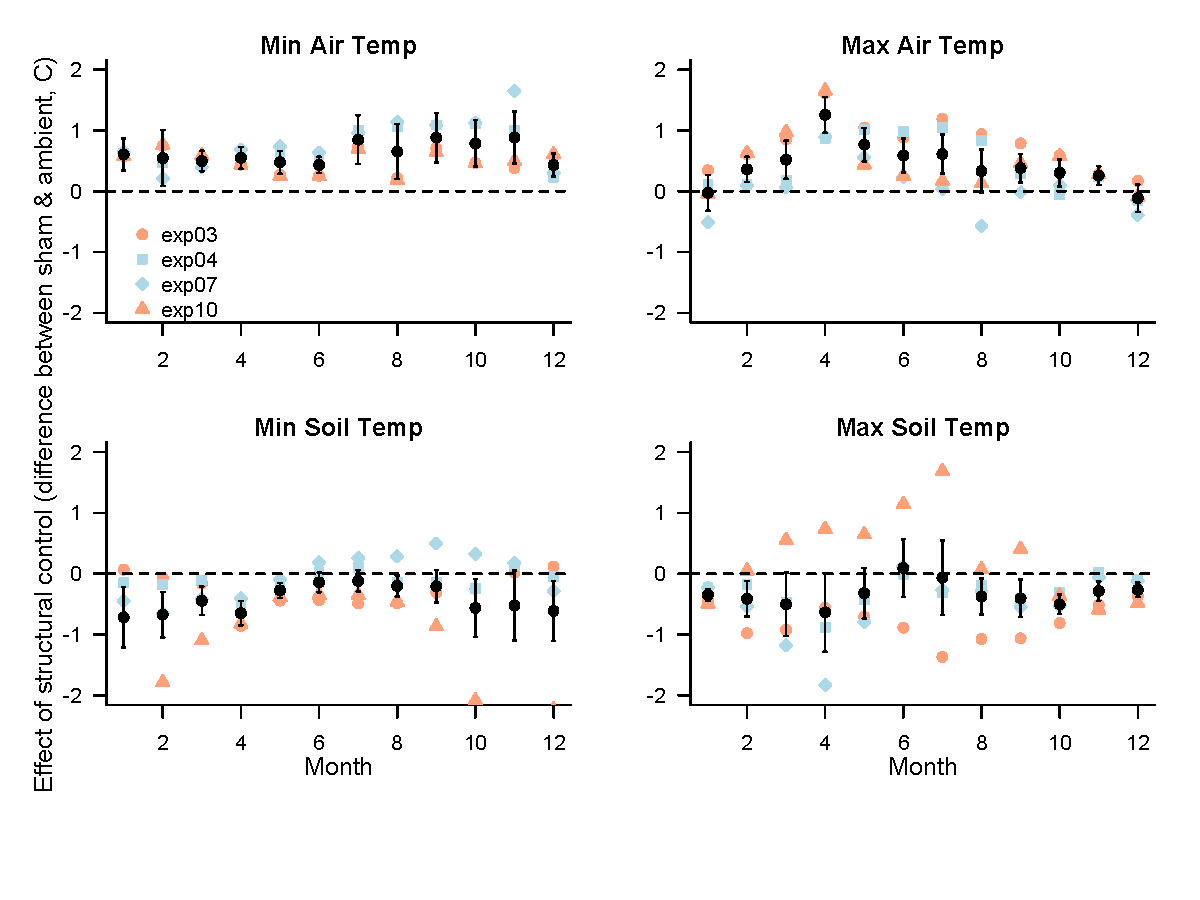
\includegraphics{../Analyses/figures/ShamVSAmbient_minmax_wranef.pdf}    
 \caption{Air temperatures were higher, whereas soil temperatures were lower, in general, in structural controls compared with ambient controls (i.e. with no control chambers or warming infrastructure in place). We show fixed effects (in black) from a mixed effects model that accounts for differences in experimental design and other factors among sites with mixed effects model including site and year (nested within site) as random effects (see Table XS, Supplemental Materials for details). Site-level random effects are shown by symbols in blue (for those at Harvard) and pink (those at Duke).}
 \label{fig:shamamb}
\end{figure}

\begin{figure}[h]
     \centering
 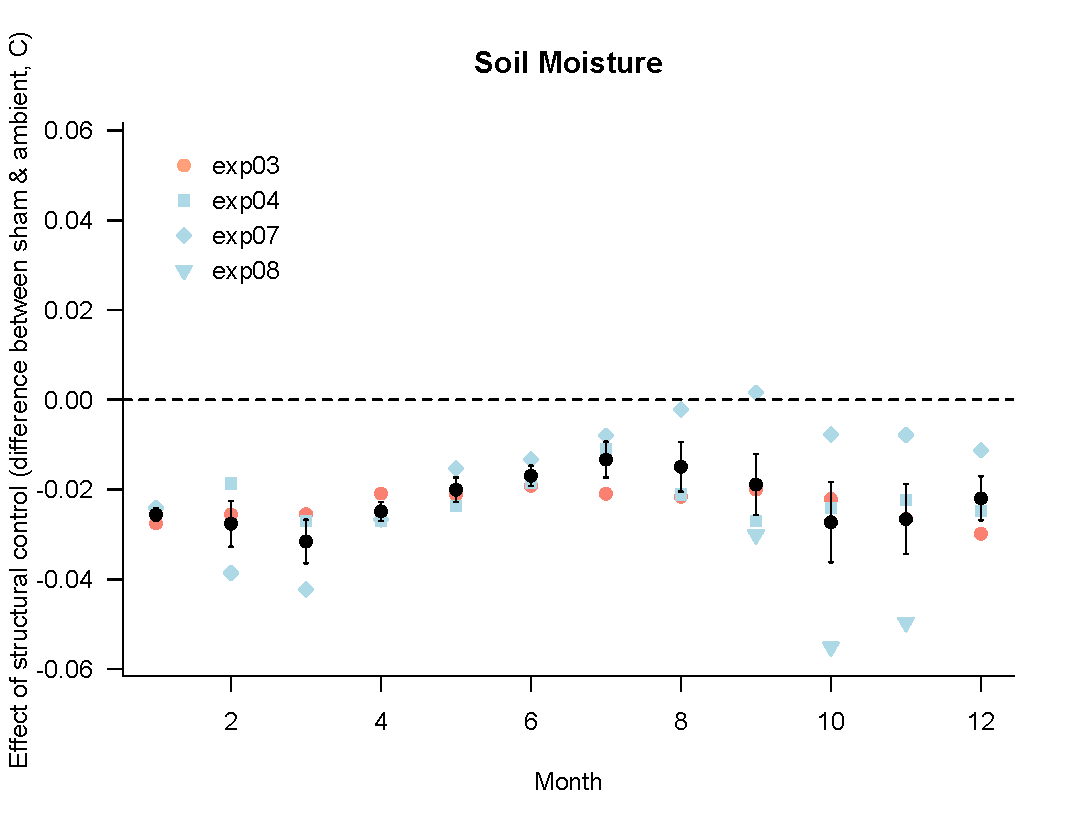
\includegraphics{../Analyses/figures/ShamVSAmbient_mois_wranef.pdf}    
 \caption{Soil moisture was lower in structural controls compared with ambient controls (i.e. with no control chambers or warming infrastructure in place). We show fixed effects (in black) from a mixed effects model that accounts for differences in experimental design and other factors among sites with mixed effects model including site and year (nested within site) as random effects (see Table XS, Supplemental Materials for details). Site-level random effects are shown by symbols in blue (for those at Harvard) and pink (those at Duke).}
\label{fig:shamamb_mois}
\end{figure}
\clearpage
 \begin{figure}[h]
     \centering
 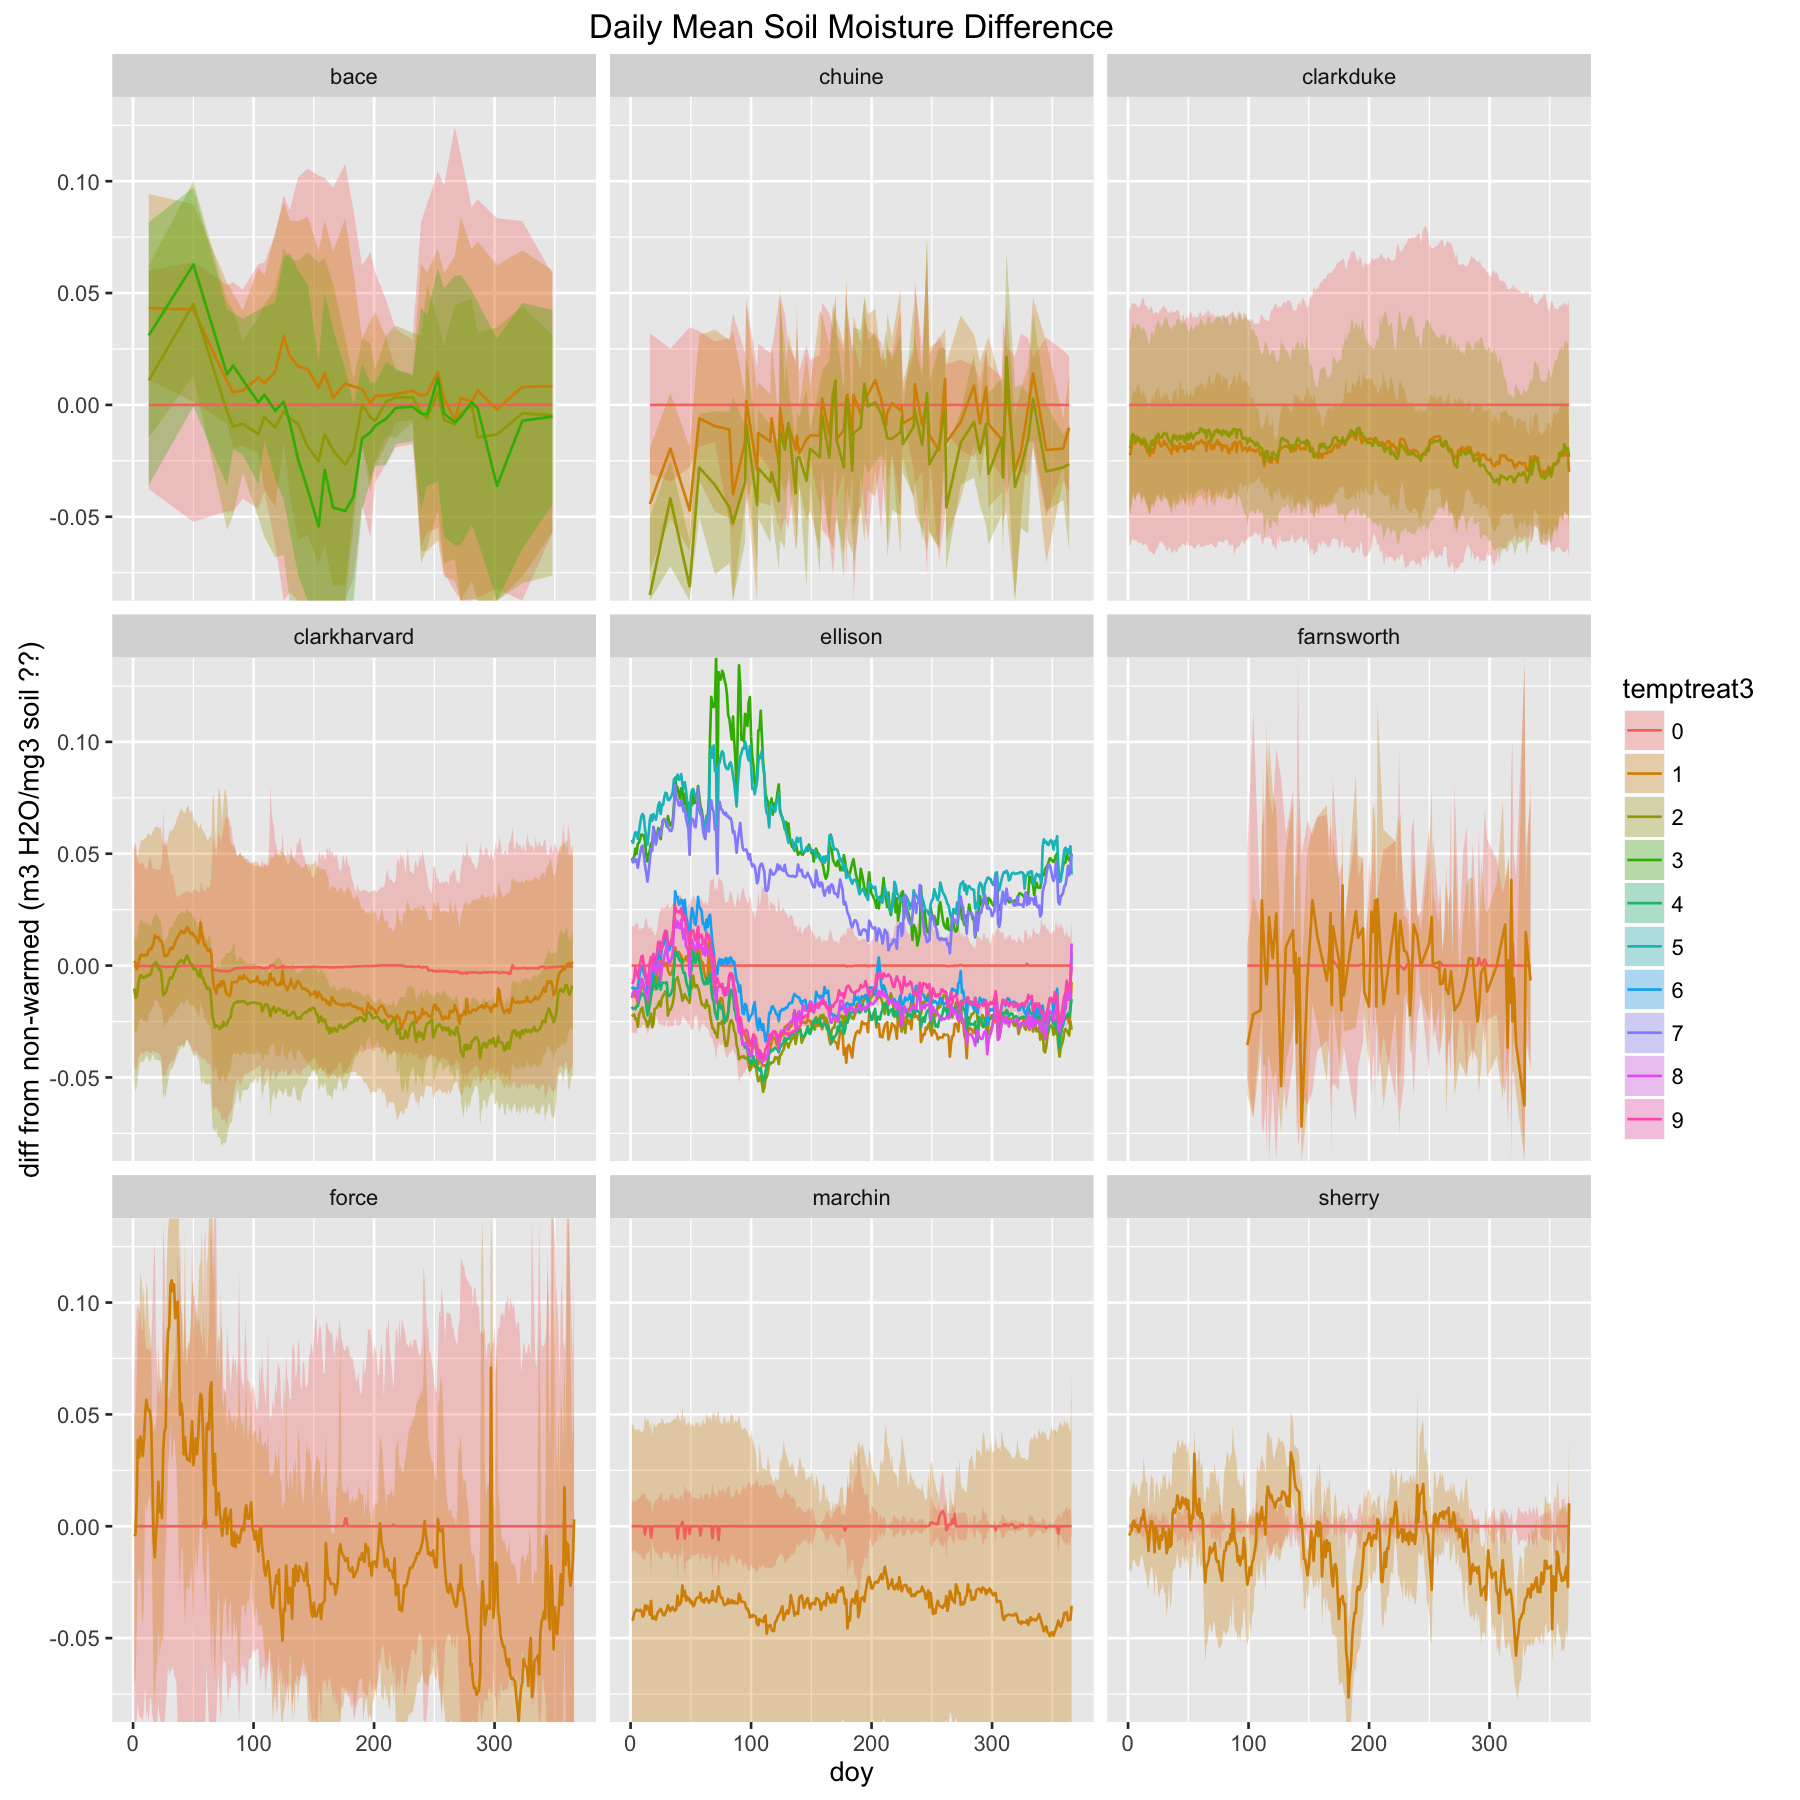
\includegraphics{../Analyses/figures/Exploratory_TimeSeries_SoilMoist_Deviation.png}    
 \caption{Time series of deviations from mean daily soil moisture in control (black line) and warming treatments with various target warming levels at 10 study sites.}
 \label{fig:mois}
 \end{figure}
 \clearpage
 \begin{figure}[h]
 \centering
 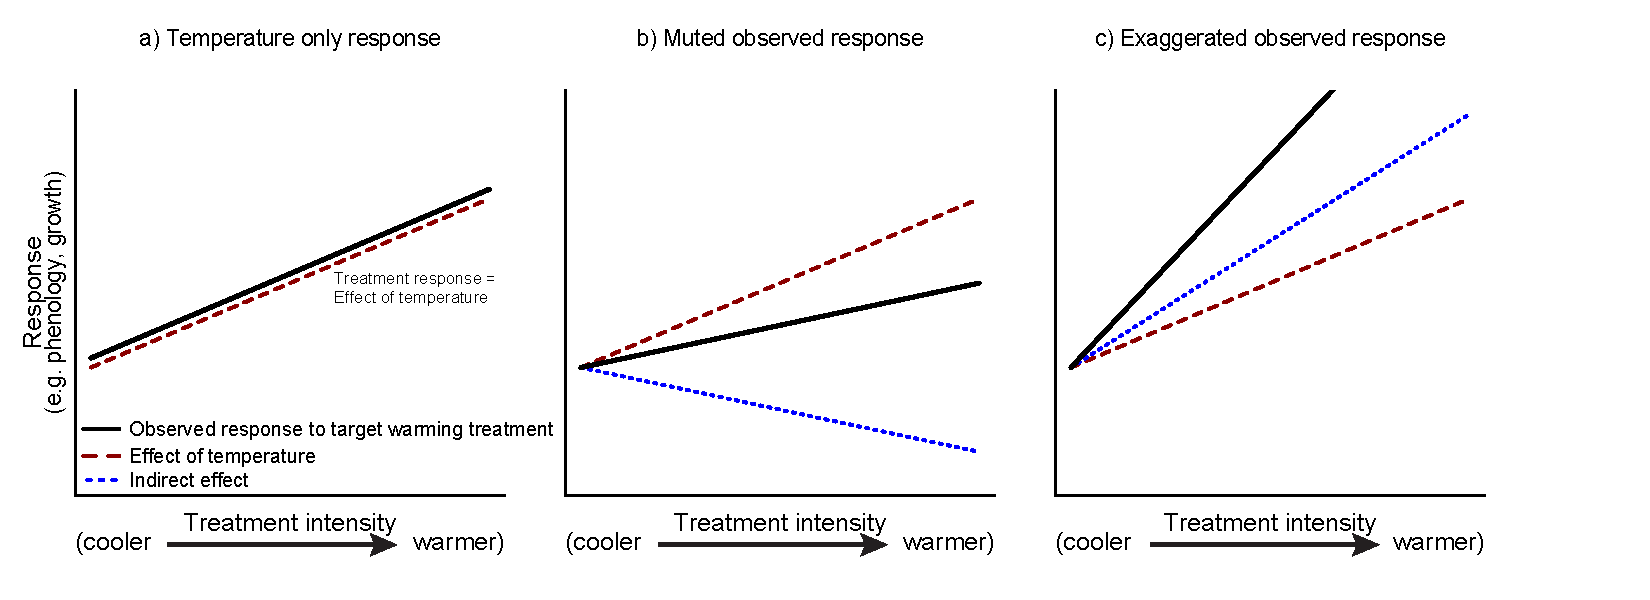
\includegraphics{../Analyses/figures/DirIndWarmingEffects.pdf}  
 \caption{Compared to direct responses to temperature alone (a), experimental warming may cause biological responses to be muted (b)or exaggerated (c), when indirect effects of experimental warming are also drivers of focal responses. For example, phenology, such as budburst which usually advances with warming, may appear to be less sensitive to warming in experiments versus observational studies \citep{wolkovich2012} because experimental warming reduces soil moisture and drying often delays phenology.}
\label{fig:biolimp}
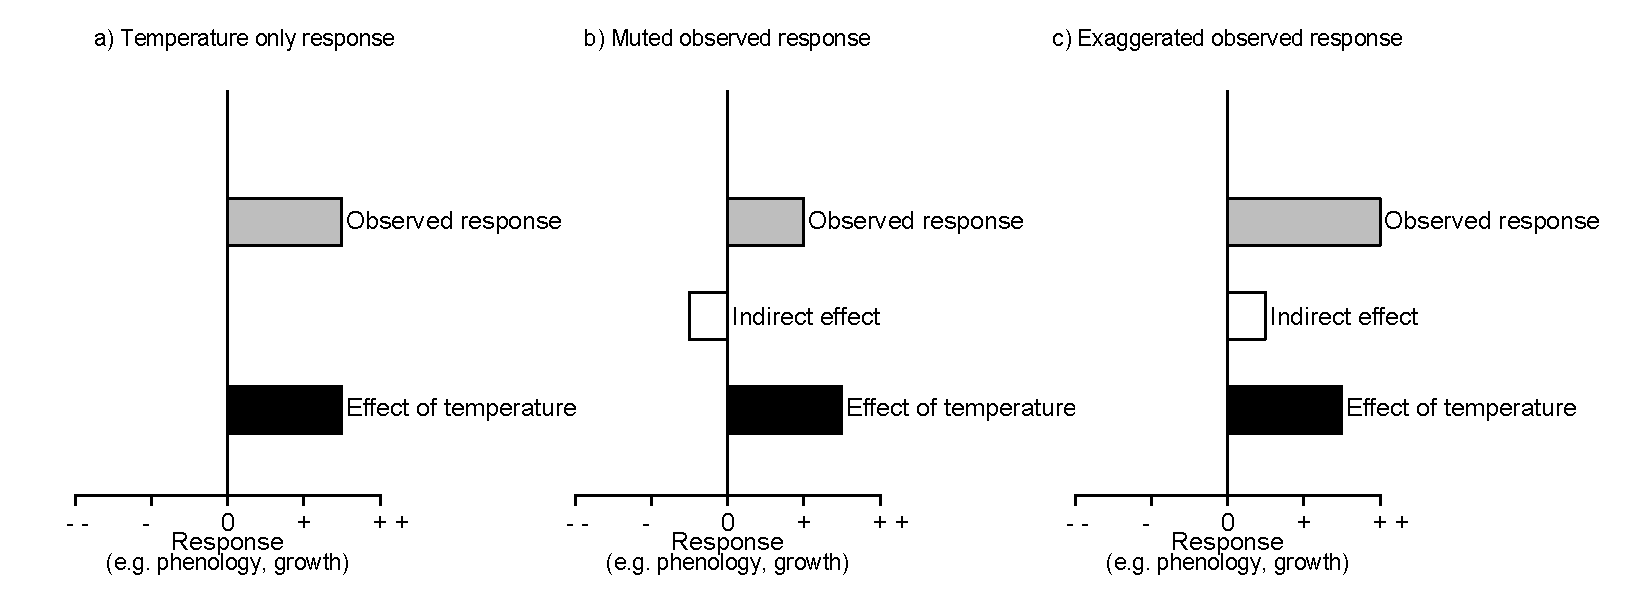
\includegraphics{../Analyses/figures/DirIndWarmingEffects_bar.pdf}   
\caption{Question for everyone (Lizzie/Ben/Miriam/Ann Marie/Aaron/Yann/Isabelle/Jeff/Christy): This is an alternative to the above figure- which do you prefer? Compared to direct responses to temperature alone (a), experimental warming may cause biological responses to be muted (b)or exaggerated (c), when indirect effects of experimental warming are also drivers of focal responses. For example, phenology, such as budburst which usually advances with warming, may appear to be less sensitive to warming in experiments versus observational studies \citep{wolkovich2012} because experimental warming reduces soil moisture and drying often delays phenology.} 
\end{figure}

%%%%%%%%%%%%%%%%%%%%%%%%%%%%%%%%%%%%%%%%
\end{document}
%%%%%%%%%%%%%%%%%%%%%%%%%%%%%%%%%%%%%%%%
